\documentclass[11pt]{article}

\usepackage{amsmath}
\usepackage{fancyhdr}
\usepackage{enumitem}
\usepackage{multirow}
\usepackage{array}
\usepackage{enumitem}
\usepackage{lipsum}
\usepackage[table]{xcolor}
\usepackage{wrapfig}
\usepackage{graphicx}

\newcommand{\ineqbox}{\fbox{\begin{minipage}[c][3ex][b]{3ex}\;\end{minipage}}}

\title{Numbers in Different Forms}
\author{Name: \rule[-5pt]{5cm}{0.5pt}}
\date{\today}

\pagestyle{fancy}
\fancyhf{}
\lhead{Page \thepage}
\rhead{\leftmark}

\begin{document}

\thispagestyle{empty}
\pagenumbering{gobble}
\maketitle
\newpage
\pagenumbering{arabic}

\section{Meaning of Each Digit}

\subsection{Basic problems}
\begin{tabular}{>{\centering\arraybackslash}p{3em} c c}
    \multirow[c]{5}{*}{27854} & 2 means & \rule[-5pt]{2.5cm}{0.5pt} \\
    & 7 means & \rule[-5pt]{2.5cm}{0.5pt} \\
    & 8 means & \rule[-5pt]{2.5cm}{0.5pt} \\
    & 5 means & \rule[-5pt]{2.5cm}{0.5pt} \\
    & 4 means & \rule[-5pt]{2.5cm}{0.5pt} \\
\end{tabular} \hspace{\stretch{1}} \begin{tabular}{>{\centering\arraybackslash}p{3em} c c}
    \multirow[c]{5}{*}{16104} & 1 means & \rule[-5pt]{2.5cm}{0.5pt} \\
    & 6 means & \rule[-5pt]{2.5cm}{0.5pt} \\
    & 1 means & \rule[-5pt]{2.5cm}{0.5pt} \\
    & 0 means & \rule[-5pt]{2.5cm}{0.5pt} \\
    & 4 means & \rule[-5pt]{2.5cm}{0.5pt} \\
\end{tabular}

\vspace{1em}

\noindent \begin{tabular}{>{\centering\arraybackslash}p{3em} c c}
    \multirow[c]{6}{*}{496813} & 4 means & \rule[-5pt]{2.5cm}{0.5pt} \\
    & 9 means & \rule[-5pt]{2.5cm}{0.5pt} \\
    & 6 means & \rule[-5pt]{2.5cm}{0.5pt} \\
    & 8 means & \rule[-5pt]{2.5cm}{0.5pt} \\
    & 1 means & \rule[-5pt]{2.5cm}{0.5pt} \\
    & 3 means & \rule[-5pt]{2.5cm}{0.5pt} \\
\end{tabular} \hspace{\stretch{1}} \begin{tabular}{>{\centering\arraybackslash}p{3em} c c}
    \multirow[c]{6}{*}{390602} & 3 means & \rule[-5pt]{2.5cm}{0.5pt} \\
    & 9 means & \rule[-5pt]{2.5cm}{0.5pt} \\
    & 0 means & \rule[-5pt]{2.5cm}{0.5pt} \\
    & 6 means & \rule[-5pt]{2.5cm}{0.5pt} \\
    & 0 means & \rule[-5pt]{2.5cm}{0.5pt} \\
    & 2 means & \rule[-5pt]{2.5cm}{0.5pt} \\
\end{tabular}

\vspace{1em}

\noindent \begin{tabular}{>{\centering\arraybackslash}p{3em} c c}
    \multirow[c]{7}{*}{3205710} & 3 means & \rule[-5pt]{2.5cm}{0.5pt} \\
    & 2 means & \rule[-5pt]{2.5cm}{0.5pt} \\
    & 0 means & \rule[-5pt]{2.5cm}{0.5pt} \\
    & 5 means & \rule[-5pt]{2.5cm}{0.5pt} \\
    & 7 means & \rule[-5pt]{2.5cm}{0.5pt} \\
    & 1 means & \rule[-5pt]{2.5cm}{0.5pt} \\
    & 0 means & \rule[-5pt]{2.5cm}{0.5pt} \\
\end{tabular} \hspace{\stretch{1}} \begin{tabular}{>{\centering\arraybackslash}p{3em} c c}
    \multirow[c]{7}{*}{9757535} & 9 means & \rule[-5pt]{2.5cm}{0.5pt} \\
    & 7 means & \rule[-5pt]{2.5cm}{0.5pt} \\
    & 5 means & \rule[-5pt]{2.5cm}{0.5pt} \\
    & 7 means & \rule[-5pt]{2.5cm}{0.5pt} \\
    & 5 means & \rule[-5pt]{2.5cm}{0.5pt} \\
    & 3 means & \rule[-5pt]{2.5cm}{0.5pt} \\
    & 5 means & \rule[-5pt]{2.5cm}{0.5pt} \\
\end{tabular}

\subsection{Challenge problems}

\begin{enumerate}
    \item Write a 5 digit number which
    \begin{enumerate}[topsep=0pt, label=\alph*.]
        \item Has 8 in its hundredth place \hspace{\stretch{1}} \rule[-5pt]{5cm}{0.5pt}
        \item Is less than 90000
    \end{enumerate}

    \vspace{1em}

    \item Write a 6 digit number which
    \begin{enumerate}[topsep=0pt, label=\alph*.]
        \item Has 7 in its thousandth place \hspace{\stretch{1}} \rule[-5pt]{5cm}{0.5pt}
    \end{enumerate}

    \vspace{1em}

    \item Write a 7 digit number which
    \begin{enumerate}[topsep=0pt, label=\alph*.]
        \item Has 0 in its thousandth place \hspace{\stretch{1}} \rule[-5pt]{5cm}{0.5pt}
        \item Contains two 2's
        \item Doesn't not contain a 9
        \item Is in between 1000000 and 2000000
    \end{enumerate}

    \vspace{1em}

    \item Write a 5 digit number which
    \begin{enumerate}[topsep=0pt, label=\alph*.]
        \item Has a 1 in its ones place \hspace{\stretch{1}} \rule[-5pt]{5cm}{0.5pt}
        \item Has a 2 in its tens place
        \item Has a 3 in its hundredth pace
        \item Has a 4 in its thousands place
        \item Has a 5 in its ten thousands place
    \end{enumerate}

    \vspace{1em}

    \item Is a 5 digit number possible which
    \begin{enumerate}[topsep=0pt, label=\alph*.]
        \item Has an even number in its ten thousands place \hspace{\stretch{1}} \rule[-5pt]{1cm}{0.5pt}
        \item Is more than 90000
    \end{enumerate}
\end{enumerate}

\section{Some Inequalities}
\fbox{\begin{minipage}{\linewidth}
    Here is a useful tip for comparing 5 digit numbers: \\

    Compare \hspace{\stretch{1}} \begin{tabular}[t]{>{\columncolor{cyan}} c c c c c}
        2 & 7 & 8 & 6 & 9 \\
        2 & 8 & 1 & 1 & 9 \\
           \multicolumn{2}{l}{$\uparrow$}    &   &   &   \\
           \multicolumn{4}{l}{same} \\
    \end{tabular} \hspace{\stretch{1}} \begin{tabular}[t]{c >{\columncolor{cyan}} c c c c}
        2 & 7 & 8 & 6 & 9 \\
        2 & 8 & 1 & 1 & 9 \\
           & \multicolumn{2}{l}{$\uparrow$} &   &   \\
           & \multicolumn{3}{l}{8 > 7} \\
    \end{tabular} \hspace{\stretch{1}} 27869 < 28133
\end{minipage}} \\ \\

\noindent Fill the following boxes with the > or < sign: \\
\renewcommand{\arraystretch}{2}
\begin{tabular}{p{0.3\linewidth} p{0.3\linewidth} p{0.3\linewidth}}
    {40971 \quad \ineqbox \;\quad 66869 } &  & { 67952 \quad \ineqbox \;\quad 85130 } \\
    {40305 \quad \ineqbox \;\quad 82696 } &  & { 35109 \quad \ineqbox \;\quad 72148 } \\
    {11566 \quad \ineqbox \;\quad 12497 } &  & { 60403 \quad \ineqbox \;\quad 78180 } \\
    {92445 \quad \ineqbox \;\quad 13895 } &  & { 16190 \quad \ineqbox \;\quad 76617 } \\
    {36953 \quad \ineqbox \;\quad 29179 } &  & { 75473 \quad \ineqbox \;\quad 76386 } \\
\end{tabular}

\section{Ordering Numbers}

\begin{tabular}{r l}
    \multirow{2}{*}{From least to greatest} & 11513, 57741, 18980, 02242, 02242 \\
    & \rule{7cm}{0.5pt} \\
\end{tabular}

\noindent \begin{tabular}{r l}
    \multirow{2}{*}{From greatest to least} & 89992, 31733, 11351, 37570, 28872 \\
    & \rule{7cm}{0.5pt} \\
\end{tabular}

\section{Combinations}
\setlength\intextsep{0pt}
\begin{wrapfigure}{r}{0.5\textwidth}
    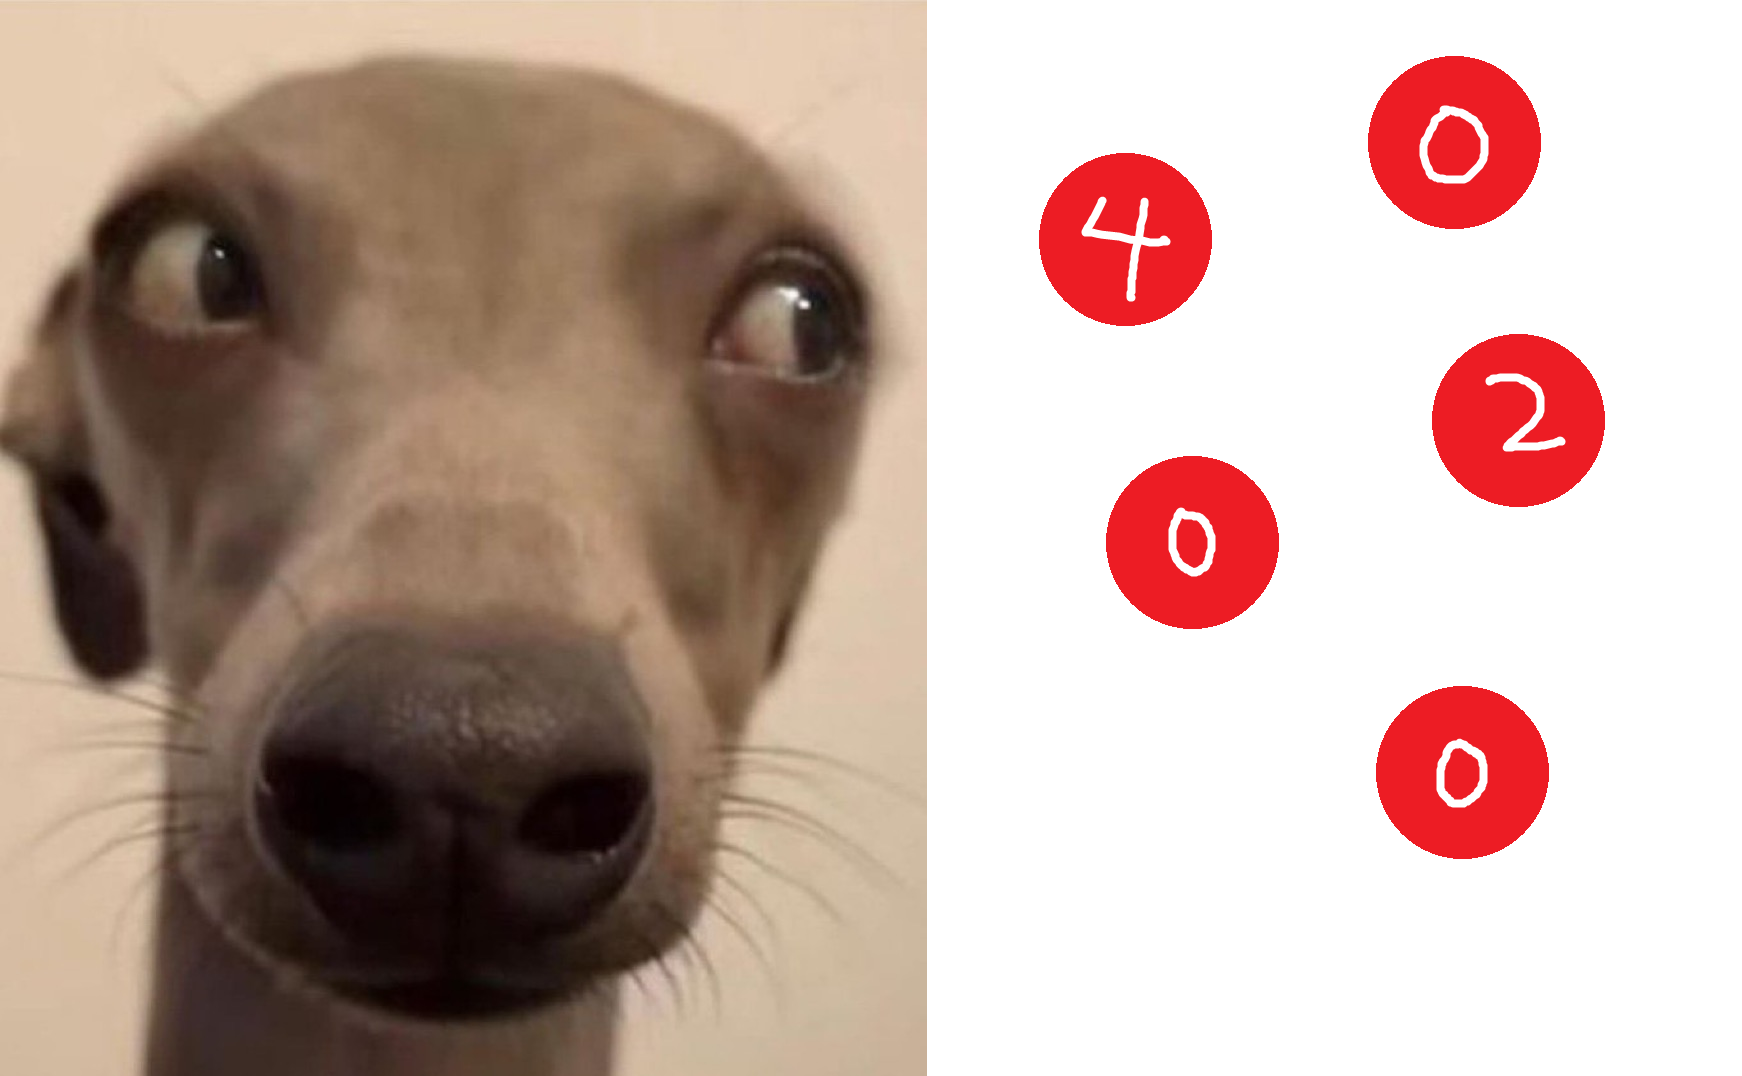
\includegraphics[width=0.45\textwidth]{math_images/dog_numbers.png}
\end{wrapfigure}

Use the numbers that the dog is looking at to form 5 digit numbers that don't begin with a 0. Then, arrange all possible number combinations from least to greatest, then from greatest to least on the respective lines:

\phantom{dog} \\

\noindent \rule{\linewidth}{0.5pt} \\

\noindent \rule{\linewidth}{0.5pt}

\end{document}